% GNUPLOT: LaTeX picture with Postscript
\begingroup
  \makeatletter
  \providecommand\color[2][]{%
    \GenericError{(gnuplot) \space\space\space\@spaces}{%
      Package color not loaded in conjunction with
      terminal option `colourtext'%
    }{See the gnuplot documentation for explanation.%
    }{Either use 'blacktext' in gnuplot or load the package
      color.sty in LaTeX.}%
    \renewcommand\color[2][]{}%
  }%
  \providecommand\includegraphics[2][]{%
    \GenericError{(gnuplot) \space\space\space\@spaces}{%
      Package graphicx or graphics not loaded%
    }{See the gnuplot documentation for explanation.%
    }{The gnuplot epslatex terminal needs graphicx.sty or graphics.sty.}%
    \renewcommand\includegraphics[2][]{}%
  }%
  \providecommand\rotatebox[2]{#2}%
  \@ifundefined{ifGPcolor}{%
    \newif\ifGPcolor
    \GPcolortrue
  }{}%
  \@ifundefined{ifGPblacktext}{%
    \newif\ifGPblacktext
    \GPblacktexttrue
  }{}%
  % define a \g@addto@macro without @ in the name:
  \let\gplgaddtomacro\g@addto@macro
  % define empty templates for all commands taking text:
  \gdef\gplbacktext{}%
  \gdef\gplfronttext{}%
  \makeatother
  \ifGPblacktext
    % no textcolor at all
    \def\colorrgb#1{}%
    \def\colorgray#1{}%
  \else
    % gray or color?
    \ifGPcolor
      \def\colorrgb#1{\color[rgb]{#1}}%
      \def\colorgray#1{\color[gray]{#1}}%
      \expandafter\def\csname LTw\endcsname{\color{white}}%
      \expandafter\def\csname LTb\endcsname{\color{black}}%
      \expandafter\def\csname LTa\endcsname{\color{black}}%
      \expandafter\def\csname LT0\endcsname{\color[rgb]{1,0,0}}%
      \expandafter\def\csname LT1\endcsname{\color[rgb]{0,1,0}}%
      \expandafter\def\csname LT2\endcsname{\color[rgb]{0,0,1}}%
      \expandafter\def\csname LT3\endcsname{\color[rgb]{1,0,1}}%
      \expandafter\def\csname LT4\endcsname{\color[rgb]{0,1,1}}%
      \expandafter\def\csname LT5\endcsname{\color[rgb]{1,1,0}}%
      \expandafter\def\csname LT6\endcsname{\color[rgb]{0,0,0}}%
      \expandafter\def\csname LT7\endcsname{\color[rgb]{1,0.3,0}}%
      \expandafter\def\csname LT8\endcsname{\color[rgb]{0.5,0.5,0.5}}%
    \else
      % gray
      \def\colorrgb#1{\color{black}}%
      \def\colorgray#1{\color[gray]{#1}}%
      \expandafter\def\csname LTw\endcsname{\color{white}}%
      \expandafter\def\csname LTb\endcsname{\color{black}}%
      \expandafter\def\csname LTa\endcsname{\color{black}}%
      \expandafter\def\csname LT0\endcsname{\color{black}}%
      \expandafter\def\csname LT1\endcsname{\color{black}}%
      \expandafter\def\csname LT2\endcsname{\color{black}}%
      \expandafter\def\csname LT3\endcsname{\color{black}}%
      \expandafter\def\csname LT4\endcsname{\color{black}}%
      \expandafter\def\csname LT5\endcsname{\color{black}}%
      \expandafter\def\csname LT6\endcsname{\color{black}}%
      \expandafter\def\csname LT7\endcsname{\color{black}}%
      \expandafter\def\csname LT8\endcsname{\color{black}}%
    \fi
  \fi
    \setlength{\unitlength}{0.0500bp}%
    \ifx\gptboxheight\undefined%
      \newlength{\gptboxheight}%
      \newlength{\gptboxwidth}%
      \newsavebox{\gptboxtext}%
    \fi%
    \setlength{\fboxrule}{0.5pt}%
    \setlength{\fboxsep}{1pt}%
\begin{picture}(10080.00,3456.00)%
    \gplgaddtomacro\gplbacktext{%
      \csname LTb\endcsname%
      \put(858,704){\makebox(0,0)[r]{\strut{}$0.99$}}%
      \put(858,1326){\makebox(0,0)[r]{\strut{}$0.995$}}%
      \put(858,1948){\makebox(0,0)[r]{\strut{}$1$}}%
      \put(858,2569){\makebox(0,0)[r]{\strut{}$1.005$}}%
      \put(858,3191){\makebox(0,0)[r]{\strut{}$1.01$}}%
      \put(990,484){\makebox(0,0){\strut{}$0$}}%
      \put(1355,484){\makebox(0,0){\strut{}$1$}}%
      \put(1721,484){\makebox(0,0){\strut{}$2$}}%
      \put(2086,484){\makebox(0,0){\strut{}$3$}}%
      \put(2451,484){\makebox(0,0){\strut{}$4$}}%
      \put(2817,484){\makebox(0,0){\strut{}$5$}}%
      \put(3182,484){\makebox(0,0){\strut{}$6$}}%
      \put(3547,484){\makebox(0,0){\strut{}$7$}}%
      \put(3912,484){\makebox(0,0){\strut{}$8$}}%
      \put(4278,484){\makebox(0,0){\strut{}$9$}}%
      \put(4643,484){\makebox(0,0){\strut{}$10$}}%
    }%
    \gplgaddtomacro\gplfronttext{%
      \csname LTb\endcsname%
      \put(2816,154){\makebox(0,0){\strut{}t, a.u.}}%
      \csname LTb\endcsname%
      \put(3788,1187){\makebox(0,0)[r]{\strut{}$\myint{\Psi}{\Psi}$}}%
    }%
    \gplgaddtomacro\gplbacktext{%
      \csname LTb\endcsname%
      \put(6118,704){\makebox(0,0)[r]{\strut{}$1.485$}}%
      \put(6118,1059){\makebox(0,0)[r]{\strut{}$1.49$}}%
      \put(6118,1415){\makebox(0,0)[r]{\strut{}$1.495$}}%
      \put(6118,1770){\makebox(0,0)[r]{\strut{}$1.5$}}%
      \put(6118,2125){\makebox(0,0)[r]{\strut{}$1.505$}}%
      \put(6118,2480){\makebox(0,0)[r]{\strut{}$1.51$}}%
      \put(6118,2836){\makebox(0,0)[r]{\strut{}$1.515$}}%
      \put(6118,3191){\makebox(0,0)[r]{\strut{}$1.52$}}%
      \put(6250,484){\makebox(0,0){\strut{}$0$}}%
      \put(6593,484){\makebox(0,0){\strut{}$1$}}%
      \put(6937,484){\makebox(0,0){\strut{}$2$}}%
      \put(7280,484){\makebox(0,0){\strut{}$3$}}%
      \put(7623,484){\makebox(0,0){\strut{}$4$}}%
      \put(7967,484){\makebox(0,0){\strut{}$5$}}%
      \put(8310,484){\makebox(0,0){\strut{}$6$}}%
      \put(8653,484){\makebox(0,0){\strut{}$7$}}%
      \put(8996,484){\makebox(0,0){\strut{}$8$}}%
      \put(9340,484){\makebox(0,0){\strut{}$9$}}%
      \put(9683,484){\makebox(0,0){\strut{}$10$}}%
    }%
    \gplgaddtomacro\gplfronttext{%
      \csname LTb\endcsname%
      \put(5216,1947){\rotatebox{-270}{\makebox(0,0){\strut{}E, a.u.}}}%
      \put(7966,154){\makebox(0,0){\strut{}t, a.u.}}%
      \csname LTb\endcsname%
      \put(8828,1169){\makebox(0,0)[r]{\strut{}$\mymean{\Psi}{\hat{H}}{\Psi}$}}%
    }%
    \gplbacktext
    \put(0,0){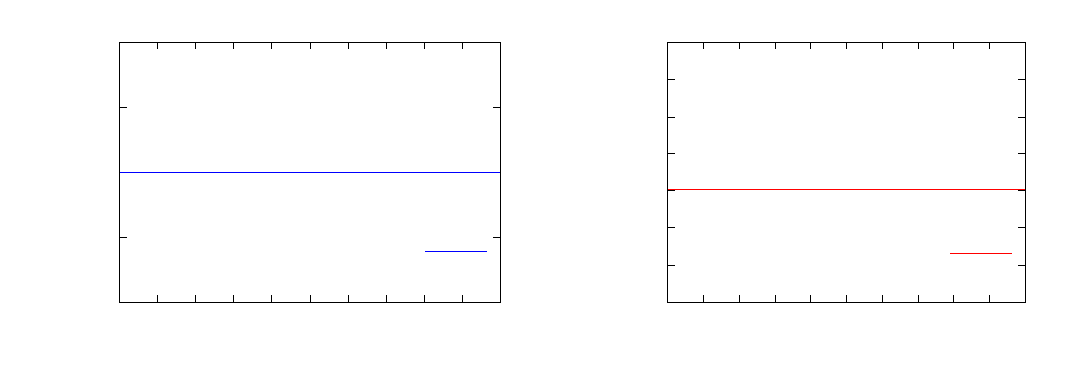
\includegraphics{results-gnuplottex-fig11}}%
    \gplfronttext
  \end{picture}%
\endgroup
